\chapter{Влияние рассеяния носителей на шероховатой поверхности на оптические свойства размерно-ограниченных систем} \label{chapt2}

\section{Межзонное и межподзонное поглощение света в квантовых системах с пониженной размерностью с учетом рассеяния на шероховатой поверхности} \label{sect2_1}

В наноструктурах зона проводимости (как и валентная зона) квантуется, поэтому возникают новые каналы поглощения (излучения) слабой электромагнитной волны в далекой инфракрасной области спектра, связанные с переходом электрона между размерно-квантованными состояниями зоны проводимости (рис. \ref{img:fig_2_1_1}).  В работе \cite{West1985} впервые наблюдалось такое поглощение света в квантовых ямах $\text{GaAs}/\text{Al}_{0.30}\text{Ga}_{0.7}\text{As}$ с толщинами $65 \AA$ и $82 \AA$ (переход I на рис. \ref{img:fig_2_1_1}).

\begin{figure}[ht] 
	\center
	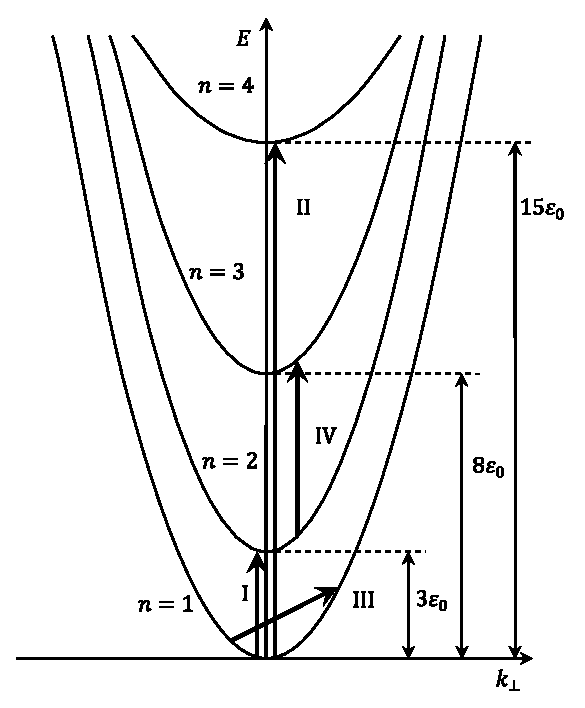
\includegraphics [scale=1] {fig_2_1_1}
	\caption{Энергетическая диаграмма для размерно-квантованной зоны проводимости в размерно-ограниченных системах. Стрелками указаны возможные оптические переходы.} 
	\label{img:fig_2_1_1} 
\end{figure}

Как показали экспериментальные исследования, частотная зависимость коэффициента поглощения света хорошо описывается лоренцовской кривой, и полуширина линии поглощения при комнатных температурах $\cong 10 \text{meV}$, что может быть связано со взаимодействием электрона с фононами. В работах \cite{Wu1994,Spector1983} исследовалось поглощение света свободными носителями в широких $(a > 10^3 \AA)$ квазидвумерных полупроводниковых структурах в нижайшем порядке теории возмущений по взаимодействию электронов с длинноволновыми акустическими колебаниями. В частности показано, что коэффициент поглощения света с ростом ширины квантовой системы уменьшается и с ростом температуры увеличивается. Однако в узких нелегированных размерно-ограниченных системах при низких температурах возможным и наиболее важным является рассеяние носителей на шероховатой поверхности. Этот механизм рассеяния определяет величину и температурную зависимость подвижности в квантовых ямах \cite{Sakaki1987}, в кремниевых инверсионных слоях \cite{Stern1980}, в которых электронный газ остается вырожденным вплоть до $T < 100 K$. Влияние шероховатой поверхности на процессы фотолюминесценции в узких $(a \geq 50 \AA)$ одиночных квантовых ямах GaAs/AlGaAs  проводилось в \cite{Gurioli1991} при $T = 4 K$. Теоретические исследования поглощения света свободными носителями с учетом взаимодействия электрона с шероховатой поверхностью проводились в \cite{Vurgaftman1999}. Рассматривался, как случай поглощения света ТМ–поляризации (электромагнитная волна распространяется вдоль оси пространственного квантования), так и случай поглощения ТЕ-поляризации (электромагнитная волна распространяется нормально к поверхности квантовой системы). В обоих случаях коэффициент поглощения света рассчитывался в нижайшем порядке по взаимодействию электрона с шероховатой поверхностью. Численные расчеты для коэффициента поглощения света справедливы естественно для частот электромагнитной волны вдали от максимума поглощения (для ТМ-поляризованной волны) и при малых взаимодействиях электрона с поверхностью исследуемой квантовой системы. Далее проводится расчет коэффициента поглощения слабой электромагнитной волны различной поляризации, результаты которого позволяют исследовать частотную зависимость поглощения света в широкой области частот и последовательно описать внутризонное поглощение света и при неслабых взаимодействиях электрона с шероховатой поверхностью.
В работах \cite{Aleshkin2002,Vorobiev2004} экспериментально, а в \cite{Thammasat1997} теоретически исследовалось межзонное поглощение света в ступенчатых квантовых ямах InGaAs/AlGaAs. При высоких уровнях возбуждения заполняются, как основная подзона, так и возбужденные состояния, что позволило наблюдать поглощение инфракрасного излучения, связанного с переходами электрона между возбужденными состояниями (переход IV на рис. \ref{img:fig_2_1_1}). При этом коэффициент поглощения достигает больших значений $(\sim 10^3 \text{cm}^{-1})$ при высоких температурах $T\sim300^{\circ}K$. Влияние поверхности на оптические характеристики в квантовых ямах GaAs/AlGaAs экспериментально исследовалось в \cite{Gurioli1991,Weisbuch1981}. В частности было показано, что учет шероховатой поверхности приводит к уширению спектров фотолюминесценции.	
			
Было проведено исследование коэффициента поглощения света $K\left(\Omega \right)$ различной поляризации, как для внутризонных переходов (переход III на рис. \ref{img:fig_2_1_1}), так и для межзонных переходов (переходы I, II) с учетом взаимодействия электронов с шероховатой поверхностью в квантовой яме. При этом коэффициент поглощения электромагнитной волны вычисляется без использования теории возмущений по взаимодействию носителей с шероховатой поверхностью, как это делалось в \cite{Vurgaftman1999}, что позволяет исследовать частотную зависимость $K(\Omega)$ в широкой области частот и сформулировать условия применимости теории возмущений.
Время релаксации при рассеянии носителей на шероховатой поверхности не зависит от волнового вектора электрона и заметным образом уменьшается с ростом $n$ и $n_1$ (см формулу в первой главе ???). Для невырожденного электронного газа, если использовать соотношения (??? главы 1) и (??? главы 1), то коэффициент поглощения света, связанный с переходом электрона из нижайшей зоны проводимости $(n=1)$ в ближайшую размерно-квантованную зону проводимости $(n_1=1)$ (переход I на рис. \ref{img:fig_2_1_1}), записывается следующим образом $(\beta _0\hbar \Omega >>1)$:

\begin{equation} \label{eq:21_10}
K \left(\Omega \right)=K_{M} \frac{1}{1+\left(\frac{\tau _{0} }{17\hbar } \Delta _{0} \right)^{2} } ;
\end{equation} 

\[
K_{M} =\frac{2^{12} e^{2} a^{5} n_{e} }{\hbar cn_{0} \pi ^{5} \gamma _{0} 3^{3} \cdot 17} ; \Delta _{0} =\hbar \Omega -3\varepsilon _{0}.
\]

 $n_{e} =N/L_{x} L_{y} $ – поверхностная плотность электронов. При записи (\ref{eq:21_10}) учитывалось, что в размерно-квантованной зоне, в которую происходит оптический переход носителя, электронов нет, поэтому  $n_{\beta } <<1$. Последнее приближение вполне справедливо, если  $3\varepsilon _{0} >>kT$, т.е. почти все электроны находятся на нижайшей размерно-квантованной зоне проводимости $(n=1)$, и, следовательно,   $\sum n_{k_{\bot } } \cong N$ ($N$– число электронов в исследуемой квантовой системе). Из (11) следует, что частотная зависимость коэффициента поглощения света описывается лоренцовой кривой с полушириной  $\delta =17\cdot 2\hbar /\tau _{0} $. Величина коэффициента поглощения электромагнитной волны при рассматриваемом механизме рассеяния существенным образом определяется толщиной квантовой ямы $\left(K_{M} \sim a^{5} \right)$ и не зависит от температуры. $K\left(\Omega \right)$  в максимуме при $n_{e} =4\cdot 10^{11} \text{cm}^{-2} $, $n_{0} =3.2$,   принимает значение   $K_{M}^{\left(\delta \right)} =0,25\cdot a_{0}^{5} /\gamma _{0} $ ($a_{0} $,$\gamma _{0}^{\frac{1}{4}} $ – измеряются в ангстремах), т.е. при  $a_{0} = 80 \AA$,  $\gamma _{0}^{\frac{1}{4}} = 10 \AA$ (именно такие значения   хорошо описывают значения подвижности   экспериментально наблюдаемые в КЯ GaAs/AlGaAs \cite{West1985}), $K_{M} =2\cdot 10^{4} \text{cm}^{-1} $). Большие значения коэффициента поглощения света позволяют надеяться на практическое использование таких размерно-квантованных систем в качестве детекторов ИК-излучения в области низких температур. Полуширина линии поглощения для рассматриваемого прямого оптического перехода при рассматриваемых выше параметрах $\delta =6.5\cdot 10^{6} \left(\gamma _{0} /a_{0}^{6} \right)\text{meV}$. Следовательно, при  $a_{0} = 60 \AA$,  $\gamma _{0}^{\frac{1}{4}} = 15 \AA$,  $\delta = 7 \text{meV}$, что безусловно, находится в области экспериментального измерения.

Для ТЕ-поляризованного излучения, возможно поглощение света только в одной размерно-квантованной зоне проводимости (переход III на рис. \ref{img:fig_2_1_1}). В случае низких температур выражение для поглощения света можно записать (см. главу I выражение (???)):
\begin{equation} \label{eq:21_20}
K(\Omega )=\frac{4\pi e^{2} n_{e} }{mcn_{0} a\hbar \beta \Omega ^{2} } \frac{\Gamma _{0} }{1+\Gamma _{0}^{2} }
\end{equation} 

Как показывают численные расчеты, соотношение (\ref{eq:21_20}) при больших $\delta $${}_{0}$ мало отличается от точного (??? главы 1). Например, при $\delta_{0} > 5$ отличие менее 10\% в широком интервале изменения $\Gamma_{0}$. Заметим, что в нижайшем приближении по взаимодействию электрона с шероховатой поверхностью $\Gamma_{0}<<1$, что соответствует обычной теории возмущений, тогда из (\ref{eq:21_20}) нетрудно получить:
\begin{equation} \label{eq:21_30}
K(\Omega )=\frac{2^{4} e^{2} n_{e} \gamma _{0} m}{\pi cn_{0} a\hbar ^{3} \beta } \left(\frac{\varepsilon _{0} }{\hbar \Omega } \right)^{3}
\end{equation} 

В рассматриваемом случае $K(\Omega )\sim \Omega ^{-3} $ и при низких температурах ($T=50^{\circ } K$) для $\gamma _{0} ^{1/4} =15 \AA$, $n_{e} =2\cdot 10^{12} \text{cm}^{-2} $, $a=50 \AA$, $K_{0} (\Omega )\cong 10\left(\frac{\varepsilon _{0} }{\hbar \Omega } \right)^{3} \text{cm}^{-1} $.

При $\Gamma _{0} >> 1$, что соответствует сильному взаимодействию электрона с шероховатой поверхностью, коэффициент внутризонного поглощения электромагнитной волны определяется соотношением:
\begin{equation} \label{eq:21_40}
K(\Omega )=\frac{2^{4} e^{2} n_{e} a}{\pi ^{3} cn_{0} \hbar } \frac{1}{\delta _{0} } \left(\frac{a^{4} }{\gamma _{0} } \right)
\end{equation} 

В рассматриваемом приближении сильной связи $a^{4} /\gamma _{0} =1$, $K(\Omega )\sim \Omega ^{-1} $ и для $\delta _{0} =10$, $a=50 \AA$, $K(\Omega )\cong 120 \text{cm}^{-1} $. Следовательно, в области низких частот для узких квантовых ям с большой флуктуацией поверхности теория возмущений при исследовании внутризонного поглощения света может оказаться несправедливой.
	

\section{Влияние лазерного излучения на оптические свойства квантовых пленок} \label{sect2_2}

Исследования резонансных явлений в физике твердого тела являются довольно привлекательными, так как в этом случае лазерное излучение приводит к заметному влиянию на кинетические явления даже при небольших интенсивностях электромагнитной волны. Примером может служить влияние инфракрасного (ИК) лазерного излучения частоты $\omega $ на коэффициент межзонного магнетопоглощения слабого света, когда $\omega $ равна циклотронной частоте $\omega _{c} $ (магнитоинфракрасный резонанс - МИКР). В этом случае резонансное ИК-излучение оказывается причиной нестационарности электронных состояний и может полностью определять форму пиков магнетопоглощения слабой электромагнитной волны при небольших интенсивностях лазерного излучения. Наиболее ярко резонансные эффекты в кинетических коэффициентах могут проявляться в размерно-квантованных системах (параболические квантовые ямы), когда частота ИК лазерного излучения равна частоте размерного квантования (размерно-инфракрасный резонанс - РИР). В частности, экспериментальное обнаружение влияния РИР на межзонное поглощение слабого света позволит не только обосновать используемые модели, но и говорить о совершенстве этих размерно-квантованных систем. В этом параграфе исследуется влияние постоянного электрического поля на межзонное поглощение слабой электромагнитной волны в режиме МИКР и РИР. Именно в постоянном электрическом поле, во-первых, наиболее отчетливо проявляются эффекты влияния на коэффициент поглощения света резонансного лазерного излучения и, во-вторых, возникают дополнительные особенности в высокочастотной области спектра поглощаемой электромагнитной волны.

Если магнитное поле $\vect{H}||OZ$, электрическое поле направлено вдоль $\vect{H}$, то гамильтониан для электрона в калибровке Ландау $A(-Hy,0,0)$ в поле лазерного излучения примет вид:

\begin{multline} \label{eq:22_10} 
\mathop{\hat{H}}\nolimits_{c} =\frac{1}{2m_{c} } \mathop{\hat{P}}\nolimits^{2} +\frac{e}{m_{c} c} (\hat{P}\xi )\sqrt{\frac{4\pi c^{2} }{V} } (\hat{b}+\mathop{\hat{b}}\nolimits^{+} )+ \\ 
+\frac{e^{2} }{2m_{c} c^{2} } \left(\frac{4\pi c^{2} }{V} \right)(\hat{b}+\mathop{\hat{b}}\nolimits^{+} )^{2} +\hbar \omega \mathop{\hat{b}}\nolimits^{+} \hat{b}+eEz\equiv \mathop{\hat{H}}\nolimits_{c}^{0} +eEz
\end{multline}
 
где $\hat{P}=\hat{p}+\frac{e}{c} \hat{A}$; $\mathop{\hat{b}}\nolimits^{+} (\hat{b})$ -- операторы рождения (уничтожения) для интенсивного лазерного излучения частоты $\omega $, поляризации $\xi $; $V$~---~объем основной области кристалла; $m_{c} $~---~эффективная масса электрона.

Коэффициент межзонного поглощения слабой электромагнитной волны частоты $\Omega $ и поляризации $\xi _{0} $ согласно формуле Кубо \cite{Kubo1957a} можно привести к виду \cite{Sokovnich2004}:
\begin{multline} \label{eq:22_20} 
K(\Omega )=\frac{4\pi e^{2} }{Vn_{0} c\hbar \Omega } \mathop{\left|\frac{p_{cv} \xi _{0} }{m_{0} } \right|}\nolimits^{2} \times  \\
\times \sum _{\beta } \int _{-\infty }^{\infty}  dt \exp \left(i\Omega t-\frac{ie^{2} E^{2} t^{3} }{6\hbar \mu } +\frac{ieEk_{z} t^{2} }{2\mu } \right)\times  \\ 
\times \mathop{\left\{<\beta ^{c} |\exp \left(\frac{it}{\hbar } \mathop{\hat{H}}\nolimits_{v}^{0} \right)\exp \left(-\frac{it}{\hbar } \mathop{\hat{H}}\nolimits_{c}^{0} \right)|\beta ^{c} >\right\}}\nolimits_{f}  
\end{multline} 

где $|\beta ^{c} >$~---~волновые функции для электронов в зоне проводимости в отсутствии электрического поля; $\beta $~--~набор квантовых чисел, описывающих состояние заряженной частицы; $p_{cv} $~---~матричный элемент оператора импульса на блоховских функциях, $\mathop{\hat{H}}\nolimits_{i}^{0} $~--~гамильтониан для электронов в магнитном поле в $i$-ой зоне ($i=c,v$); $\{ \} _{f} $~---~описывает усреднение по системе свободного фотонного поля \cite{Glauber1963,Klauder1968}. 

Далее исследуем случай, когда электрическое поле $E_{0} $ линейно--поляризованного лазерного излучения перпендикулярно $H$, т.е. лазерное излучение распространяется вдоль $H$. Именно в такой поляризации интенсивная электромагнитная волна смешивает ближайшие уровни Ландау. Дальнейшие расчеты, для простоты, проводятся в резонансном приближении $\omega _{c} =eH/(m_{c} c)=\omega $ (магнитоинфрокрасный резонанс МИКР), и, поэтому не учитывается взаимодействие дырок с лазерным излучением ($\omega _{v} =eH/(m_{v} c)\ne \omega $, $m_{v} \gg m_{c} $). В рассматриваемом приближении третьим слагаемым в \eqref{eq:22_10}, описывающим двухфотонные процессы, пренебрегаем. В результате, проводя расчет методом, использованным в \cite{Sinyavskii1974,Sinyavskii2002}, нетрудно получить: 
\begin{multline} \label{eq:22_30} 
K(\Omega )=\frac{2e^{2} }{n_{0} c\hbar R^{2} } \mathop{\left|\frac{p_{cv} \xi _{0} }{m_{0} } \right|}\nolimits^{2} \sqrt{\frac{2\mu }{\pi \hbar \omega } } \frac{1}{\gamma ^{{\tfrac{1}{4}} } } \times \\
\times \sum _{n} \int _{0}^{\infty } \frac{d\tau }{\sqrt{\tau } } \cos \left(a\tau ^{3} -\Delta _{n} \tau +\frac{\pi }{4} \right)\exp \left(-\frac{\tau ^{2} }{2} \right)L_{n} (\tau ^{2} )
\end{multline} 

где 
\[
\Delta _{n} =\frac{\hbar \Omega -E_{g} -\hbar \omega ^{*} \left(n+{\tfrac{1}{2}} \right)}{\hbar \omega \sqrt{\gamma } } ;\; \; a=\frac{e^{2} E^{2} }{24\mu \omega ^{3} \hbar \gamma ^{{\tfrac{3}{2}} } } ;\; \; \gamma =\frac{e^{2} E_{0}^{2} }{8\mu \hbar \omega ^{3} } ;
\] 
$\mu ^{-1} =m_{c}^{-1} +m_{v}^{-1} ;$~~$\omega ^{*} =\omega _{c} +\omega _{v} ;$~~$L_{n} (z)$~---~полиномы Лагерра; $E_{g} $~---~ширина запрещенной зоны; $n$~---~номер уровня Ландау. 

\noindent Как непосредственно следует из \eqref{eq:22_30}, в поле резонансного ИК лазерного излучения $(\omega _{c} =\omega )$ возникает затухание гауссовского типа $\exp \left(-\tau ^{2} /2\right)$, т.е. лазерное излучение приводит к нестационарности электронных состояний. При записи \eqref{eq:22_30} пренебрегалось влиянием электрон--фононного взаимодействия на форму линии магнетопоглощения. Как показали детальные исследования в работе \cite{Sinyavskii1976}, это вполне оправдано для реальных полупроводниковых материалов даже при небольших интенсивностях резонансного ИК лазерного излучения. 

На рис. \ref{img:fig_2_2_1} представлены частотные зависимости линии магнетопоглощения в относительных единицах для $n=0$, т.е. для оптических переходов между нижайшими уровнями Ландау валентной зоны и зоны проводимости при различных значениях постоянного электрического поля. Кривые 1, 2, 3 получены соответственно для $a=0$, $a=0.4$, $a=0.8$.

\begin{figure}[ht] 
	\center
	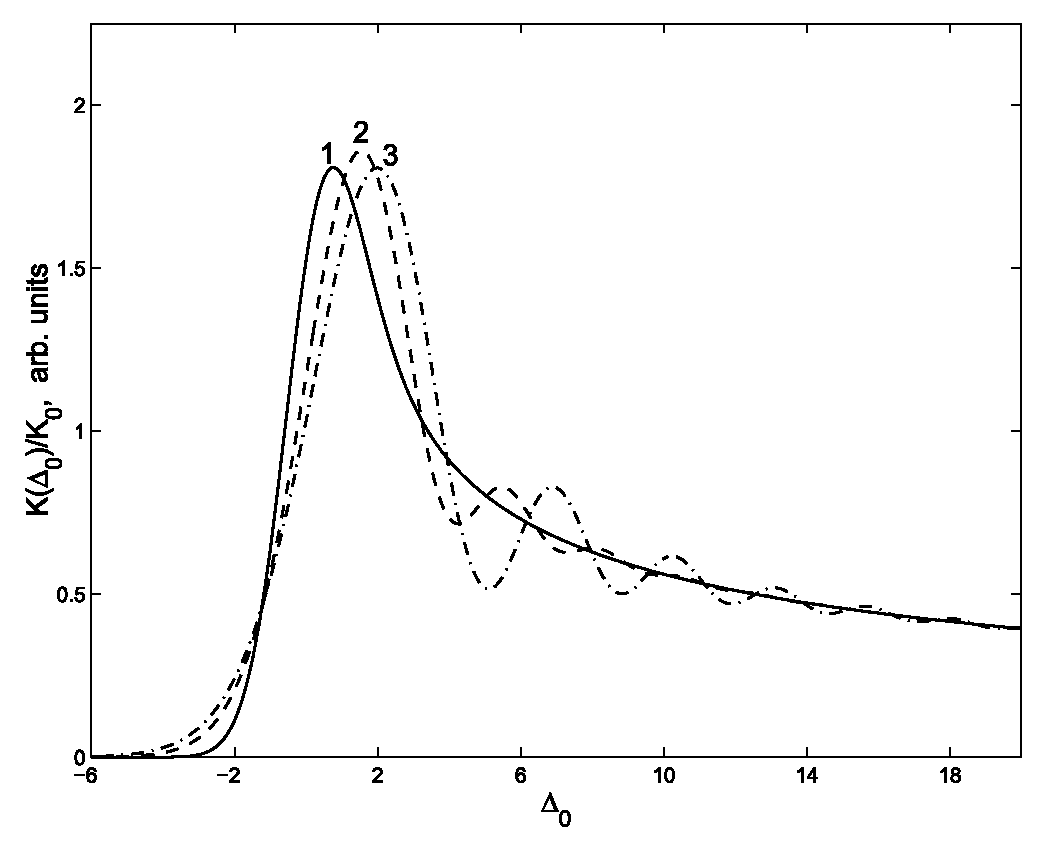
\includegraphics [scale=1] {fig_2_2_1}
	\caption{Частотная зависимость первого пика магнетопоглощения в режиме магнитоинфракрасного резонанса. Кривые 1, 2, 3 получены соответственно для $a=0$; $a=0.4$; $a=0.8$.} 
	\label{img:fig_2_2_1} 
\end{figure}

Из представленных результатов видно, что с ростом напряженности электрического поля величина первого пика магнетопоглощения уменьшается, полуширина увеличивается, и в высокочастотной области возникают осцилляции коэффициента поглощения света. При переходе электрона на первый уровень Ландау (в формуле \eqref{eq:22_30} $n=1$) частотная зависимость второго пика магнетопоглощения описывается двумя пиками, причем величина длинноволнового пика меньше величины пика в высокочастотной области спектра (рис. \ref{img:fig_2_2_2}, кривая 1 получена при $a=0$). С ростом напряженности однородного электрического поля величина коротковолнового пика уменьшается, и в высокочастотной области возникают характерные осцилляции коэффициента поглощения света (кривые 2, 3 на рис. \ref{img:fig_2_2_2} получены при $a=0.4$, $a=0.8$ соответственно). 

\begin{figure}[ht] 
	\center
	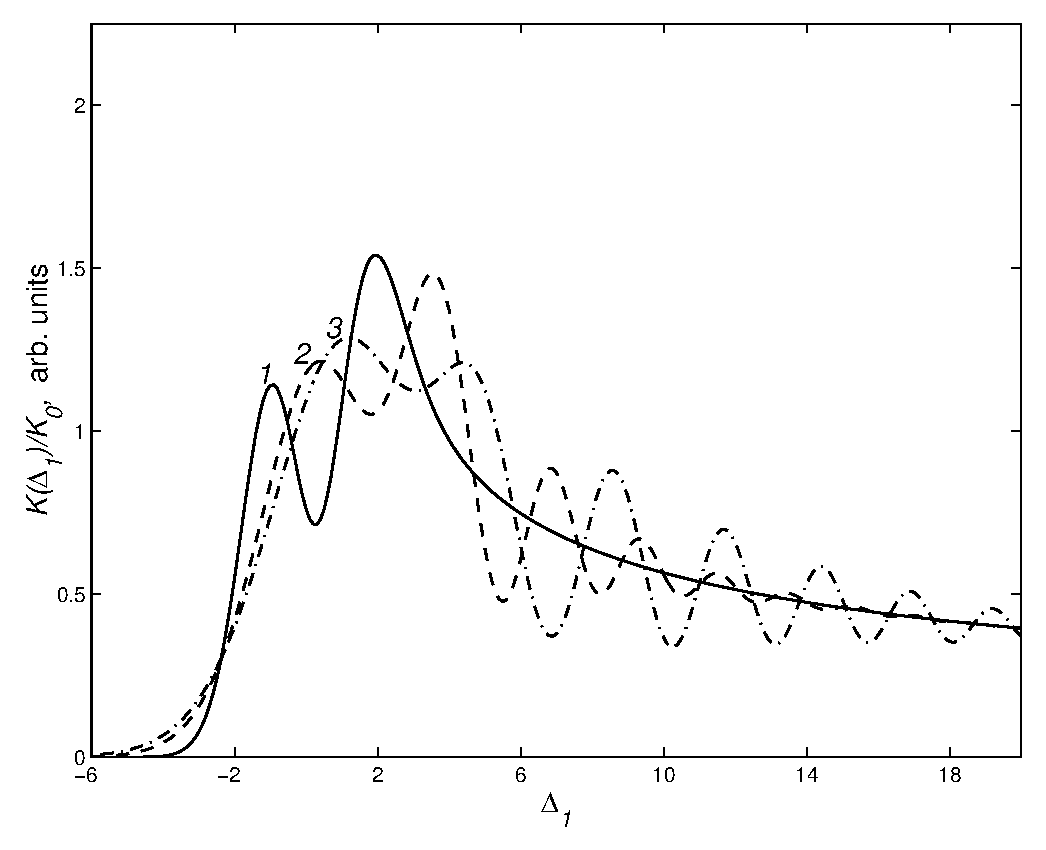
\includegraphics [scale=1] {fig_2_2_2}
	\caption{Частотная зависимость второго пика магнето-поглощения в режиме магнитоинфракрасного резонанса. Кривые 1, 2, 3 получены соответственно для $a=0$; $a=0.4$; $a=0.8$.} 
	\label{img:fig_2_2_2} 
\end{figure}

Теперь рассмотрим межзонное поглощение слабой электромагнитной волны в параболических квантовых ямах, в которых благодаря размерному квантованию возникают эквидистантные зоны проводимости и валентные зоны. Если электрическое поле линейно-поляризованного излучения направлено вдоль оси пространственного квантования, то инфракрасное лазерное излучение смешивает ближайшие эквидистантные зоны. Вычислим коэффициент межзонного поглощения слабого света, когда частота лазерного излучения $\omega $ равна частоте размерного квантования $\omega _{c} $ в зоне проводимости (размерно-инфракрасный резонанс -- РИР), а напряженность $E$ постоянного электрического поля направлена параллельно поверхности параболической квантовой ямы (ПКЯ). Коэффициент поглощения $K(\Omega )$ вычисляется так же, как это было сделано выше и с учетом тех же приближений принимает следующий вид: 
\begin{multline} \label{eq:22_40} 
K(\Omega )=K_{0} \sum _{n} \, V_{n}^{2} \times  \\
\times \left\{\frac{\pi }{2} +\int _{0}^{\infty } dt \exp \left(-\frac{x^{2} }{2} \right)L_{n} \left(x^{2} \right)\frac{\sin \left[x\left(\Delta _{n} -\delta x^{2} \right)\right]}{x} \right\}
\end{multline} 
где 
\[\Delta _{n} =\frac{\hbar \Omega -E_{g} -\hbar \omega ^{*} \left(n+{\tfrac{1}{2}} \right)}{\hbar \sqrt{\gamma } } ;\; \; \omega ^{*} =\omega _{c} +\omega _{v} ;\] 
$\hbar \omega _{v} $~---~энергия размерного квантования в валентной зоне, $V_{n} $~---~матричный элемент волновых функций электрона в зоне проводимости и в валентной зоне для ПКЯ \cite{Sinyavskii2002}. В отсутствии постоянного электрического поля $(E=0)$ \eqref{eq:22_40} переходит в выражение для межзонного поглощения света в режиме РИР, полученного в \cite{Sinyavskii2002}. В частном случае 
\[V_{0} =\mathop{\left(\lambda _{c} \lambda _{v} \right)}\nolimits^{{\tfrac{1}{4}} } \sqrt{\frac{2}{\lambda _{c} +\lambda _{v} } } ;\; \; V_{1} =2\sqrt{2} \frac{\mathop{\left(\lambda _{c} \lambda _{v} \right)}\nolimits^{{\tfrac{3}{4}} } }{\mathop{\left(\lambda _{c} +\lambda _{v} \right)}\nolimits^{{\tfrac{3}{2}} } } ;\; \; \lambda _{i} =\frac{m_{i} \omega ^{i} }{\hbar } (i=c,v).\] 
Для типичных параметров ПКЯ GaAs-AlGaAS $\lambda _{c} /\lambda _{v} =0.47$ ($m_{c} =0.06m_{0} ,$ $m_{v} =0.4m_{0} $). На рис. \ref{img:fig_2_2_3} приведена частотная зависимость коэффициента межзонного поглощения света (в относительных единицах) при переходе электрона из нулевого (первого $n=1$) размерно-квантованного состояния валентной зоны на нулевое $n=0$ (первое $n=1$) размерно-квантованное состояние зоны проводимости. Кривая 1 описывает частотную зависимость коэффициента поглощения в отсутствии постоянного электрического поля \cite{Sinyavskii2002}. Кривая 2 получена при $a=0.4$, кривая 3 при $a=0.8$. Из рис. \ref{img:fig_2_2_3} видно, что постоянное продольное электрическое поле существенным образом влияет на межзонный коэффициент поглощения света. При этом в электрическом поле возможно заметное поглощение в длинноволновой области спектра, а в высокочастотной области поглощение света определяется характерной осцилляционной зависимостью от частоты. С ростом напряженности постоянного электрического поля осцилляции становятся наиболее отчетливыми. 
\begin{figure}[ht] 
	\center
	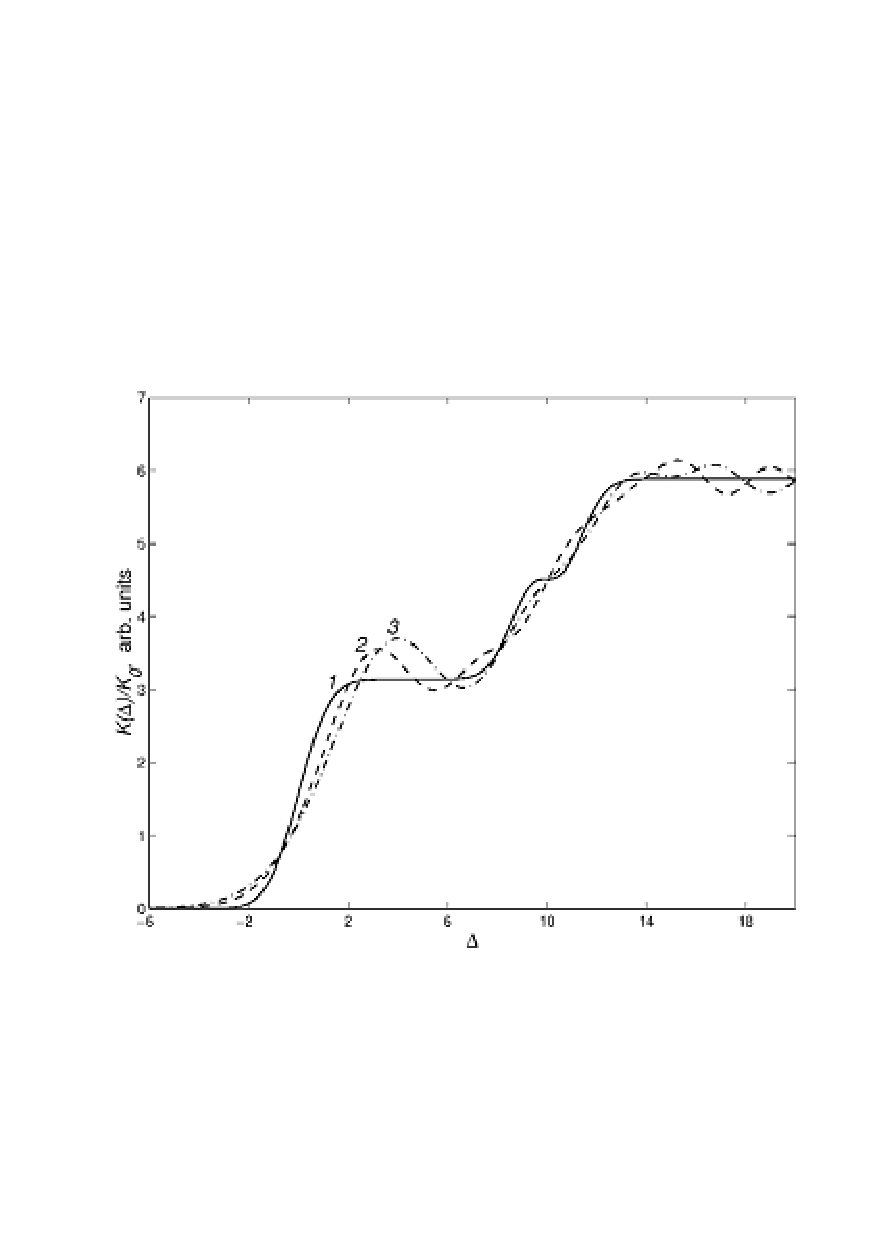
\includegraphics [scale=1] {fig_2_2_3}
	\caption{Частотная зависимость межзонного поглощения света в режиме размерноинфракрасного резонанса. Кривые 1, 2, 3 получены соответственно для $a=0$; $a=0.4$; $a=0.8$.} 
	\label{img:fig_2_2_3} 
\end{figure}


\section{Оптические свойства квантовых проволок в присутствии резонансного лазерного излучения} \label{sect2_3}

Теперь исследуем явления, связанные с МИКР и размерно-инфракрасным резонансом (РИР) в квантовой проволоке в однородном магнитом поле ${\mathbf B}$, направленном перпендикулярно оси исследуемой наноструктуры с учетом взаимодействия носителей с шероховатой поверхностью. Такие одномерные структуры интересны тем, что имеют особенности в плотности энергетических состояний, приводящие к особенностям оптических свойств. Энергетический спектр электрона в параболической нанопроволоке известен \cite{Hashimzade2005}:
\[
E_{\alpha }=\frac{{\hbar }^2k^2_x}{2m^*_e}+\hbar \Omega_e\left(n+\frac{1}{2}\right)+\hbar {\omega }_e\left(m+\frac{1}{2}\right)
\] 
\[
m^*_e=m_e{\left(\frac{\Omega_e}{{\omega }_e}\right)}^2,\ \ \Omega_e={\left[{\omega }^2_e+{{\omega }_с}^2\right]}^{1/2},\ \ {\omega }_с=\frac{eB}{m_ec\ }
\] 
$\hbar {\omega }_e$~--~энергия размерного квантования электрона массы $m_e$ в зоне проводимости, ${\omega }_с$~--~циклотронная частота. Аналогично можно записать энергию для электрона в валентной зоне.

\begin{figure}[ht] 
	\center
	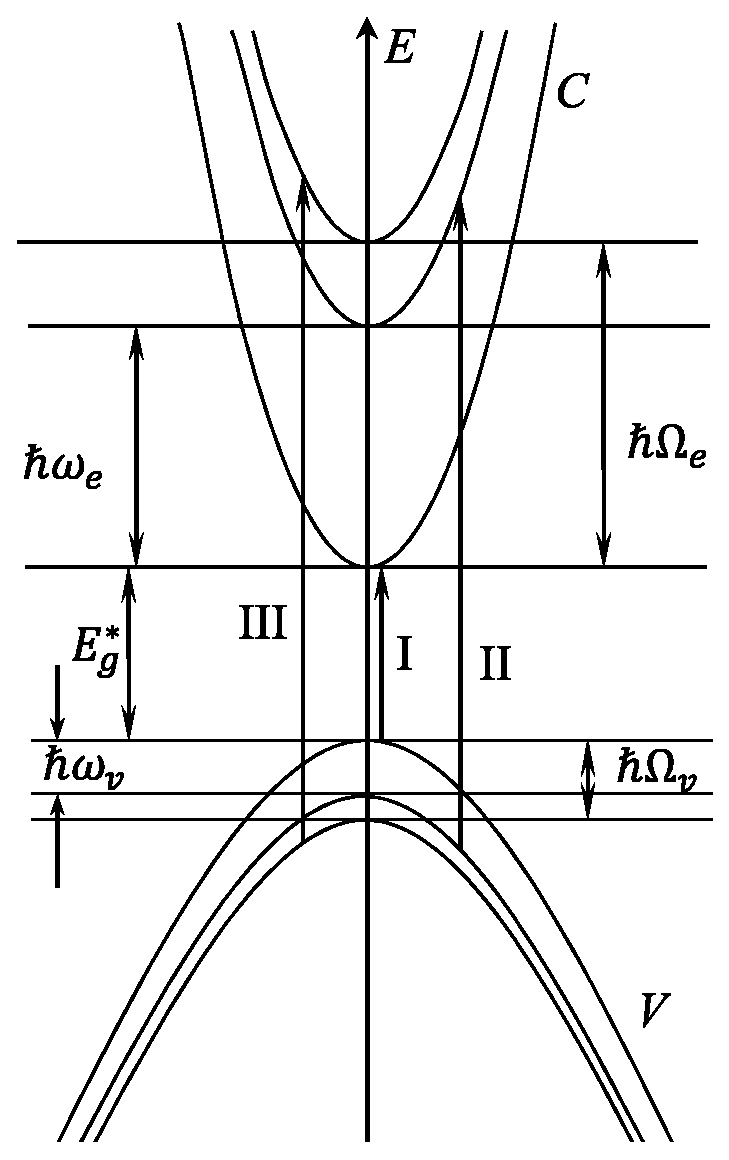
\includegraphics [scale=1] {fig_2_3_1}
	\caption{Схема энергетических зон полупроводниковой квантовой проволоки в поперечном магнитном поле и оптические переходы.} 
	\label{img:fig_2_3_1} 
\end{figure}

Будем исследовать оптические свойства полупроводниковых квантовых проволок (КП), схема энергетических зон которых изображена на рис. \ref{img:fig_2_3_1} $E^*_g$ -- ширина запрещенной зоны КП в магнитном поле, $\omega_v, \Omega_v$~---~соответственно частота размерного квантования и гибридная частота носителей в валентной зоне.

Вычислять коэффициент межзонного поглощения слабой электромагнитной волны в поле лазерного излучения, будем в случае, когда его частота $\omega_L$ равна $\omega_e$ частоте размерного квантования (РИР) или $\Omega_e$ (магнитно-инфракрасный резонанс). Так как для типичных полупроводниковых наноструктур эффективная масса электронов в зоне проводимости значительно меньше массы дырок ($m_e\ll m_v$), то взаимодействием интенсивного ИК излучения с электронами в валентной зоне в дальнейшем пренебрегаем ($\omega_e\gg \omega_v\ $).

Гамильтониан в представлении вторичного квантования для электронов в зоне проводимости в состоянии $\alpha $ в поле одномодового лазерного излучения поляризацией ${\mathbf \xi }$ записывается в следующем виде:
\begin{equation} \label{eq:23_10} 
\hat{H}=\sum_{\alpha }{{\varepsilon }_{\alpha }a^+_{\alpha }a_{\alpha }}+\ \hbar {\omega }_Lb^+b+{\left[\frac{2\pi \hbar e^2}{V{\omega }_L}\right]}^{\frac{1}{2}}{\sum_{\alpha {\alpha }_1}{\left|\frac{{{\mathbf P}}_{\alpha {\alpha }_1}{\mathbf \xi }}{m_e}\right|}}^2a^+_{\alpha }a_{{\alpha }_1}(b^++b)
\end{equation}

Здесь $a^+_{\alpha }\ (a_{\alpha })$, $b^+\ (b)$ -- операторы рождения (уничтожения) электронов в состоянии $\alpha $ и фотонов.

Расчет матричных элементов оператора импульса $\vect{P}_{\alpha\alpha_1}$ на волновых функциях квантовой параболической проволоки в продольном магнитном поле \cite{Hashimzade2005} не представляет труда. В результате:

\begin{equation} \label{eq:23_20}
\begin{aligned}
&{\left|\vect{P}^X_{\alpha \beta }\right|}^2=\frac{{\delta }^2}{{\left({1+\delta }^2\right)}^{1/2}}{\left|P^Y_{\alpha \beta }\right|}^2, \delta =\left(\frac{{\omega }_с}{{\omega }_e}\right),\\
&{\left|\vect{P}^Y_{\alpha \beta }\right|}^2=\frac{\hbar {\omega }_e{{\left({1+\delta }^2\right)}^{1/2}m}_e}{2} \delta_{k_x,k_x^{'}}\delta_{m,m_1} \left\{n{\delta }_{n,n_1+1}+\left(n+1\right){\delta }_{n,n_1-1}\right\},\\
&{\left|\vect{P}^Z_{\alpha \beta }\right|}^2=\frac{\hbar {\omega }_e m_e}{2}{\delta }_{k_{x},k_x^{'}} {\delta }_{n,n_1}\left\{m{\delta }_{m,m_1+1}+\left(m+1\right){\delta }_{m,m_1-1}\right\}.
\end{aligned}
\end{equation}

Из выражения \eqref{eq:23_20} следует, что линейно X-поляризованная волна лазерного излучения (электромагнитная волна распространяется перпендикулярно оси нанопроволоки) в отсутствии магнитного поля $\left(\delta =0\right)\ $ не взаимодействует с зонными носителями. Согласно \eqref{eq:23_20} линейно Y-поляризованная волна (лазерное излучение распространяется вдоль оси квантовой проволоки) смешивает гибридные состояния ($\hbar {\omega }_L=\hbar \Omega_e$), а Z-поляризованная волна (напряженность электрического поля лазерного излучения $\vect{E}\bot \vect{B}$) смешивает только размерно-квантованные состояния ($\hbar {\omega }_L=\hbar {\omega }_e)$.

Расчет коэффициента межзонного поглощения слабой электромагнитной волны частоты $\Omega$ в поле резонансного лазерного излучения для квантовых проволок производился с использованием формулы Кубо \cite{Kubo1957a} и методики, развитой в \cite{Sinyavskii1974}. В результате при ${\omega }_L=\Omega_e$ (резонансный случай) для стабильно генерирующего ИК лазерного излучения Y-поляризации получаем:
\begin{multline} \label{eq:23_30}
K\left(\Omega\right)=K_0{\sum_{nm}{\left|\left\langle {\alpha }_c\mathrel{\left|\vphantom{{\alpha }_c {\alpha }_v}\right.\kern-\nulldelimiterspace}{\alpha }_v\right\rangle \right|}}^2\int^{\infty }_{-\infty }{dk_x}\int^{\infty }_{-\infty }{dt}e^{-at^2}e^{-\frac{{\gamma }_0\left|t\right|}{\left|k_x\right|}}L_n\left(2at^2\right)\times\\
\times {\exp \left\{\frac{it}{\hbar }\left[\hbar \Omega-E^*_g-\frac{{\hbar }^2k^2_x}{2{\mu }^*\ }-m\left(\hbar {\omega }_e+\hbar {\omega }_v\right)-n\left(\hbar \Omega_e+\hbar \Omega_v\right)\right]\right\}\ }
\end{multline}
\[
K_0=\frac{\hbar \Omega e^2}{4{\mu }^*E^*_gn_0cs}, 
a=\frac{e^2E^2}{8m_e\hbar \Omega_e}, \frac{1}{{\mu }^*}=\frac{1}{m^*_e}+\frac{1}{m^*_v}, m^*_v=m_v{\left(\frac{\Omega_v}{{\omega }_v}\right)}^2
\] 
$\left\langle {\alpha }_c\mathrel{\left|\vphantom{{\alpha }_c {\alpha }_v}\right.\kern-\nulldelimiterspace}{\alpha }_v\right\rangle $ -- матричный элемент сглаженных волновых функций электрона в зоне проводимости и в валентной зоне, $L_n\left(z\right)$ -- полиномы Лаггера, $E$ -- напряженность электрического поля лазерного излучения, $s$ -- сечение квантовой проволоки. 

При записи \eqref{eq:23_30} учитывалось взаимодействие носителей с шероховатой поверхностью или с длинноволновыми акустическими фононами в приближении времени релаксации \cite{Khamidullin2002}. ${{\gamma }_0}/{\left|k_x\right|}$~--~описывает вероятность рассеяния электронов в единицу времени или на шероховатой поверхности \cite{Karapetyan2012} или упругое рассеяние на акустических фононах \cite{Khamidullin2006}.

Запишем коэффициент поглощения света, связанный с переходом электрона из нижайшей валентной зоны ($m=n=0$) в нижайшую размерно-квантованную зону проводимости ($n=m=0$). (Оптический переход I на рис. \ref{img:fig_2_3_1}) Интегрирование по t в  \eqref{eq:23_30} проводится точно, в результате, после замены
\[
\frac{{\hbar }^2k^2_x}{2{\mu }^*}=\hbar {\omega }_fx^2, \left({\omega }^3_f=\frac{\hbar {\gamma }^2_0}{2{\mu }^*}\right)
\] 
соотношение  \eqref{eq:23_30} записывается в виде $\left(L_0\left(z\right)=1\right)$:
\begin{equation} \label{eq:23_40}
K\left(\Omega\right)=K_0\sum_{nm}{ {\lvert\langle \alpha_c | \alpha_v \rangle\rvert}^2 {\left[\frac{8\pi {\mu }^*{\omega }_f}{\hbar a}\right]}^{\frac{1}{2}} \mathrm{Re} \int\limits_{0}^\infty {dx e^{f^2\left(x\right)}\left[1-\Phi \left(f\left(x\right)\right)\right]}}
\end{equation}
\[
\Phi \left(z\right)=\frac{2}{\sqrt{\pi }}\int\limits_{0}^z {e^{-{\tau}^2}}d\tau ,
\] 
\[
f\left(x\right)={\left(\frac{{\omega }^2_f}{4a}\right)}^{\frac{1}{2}}\frac{1}{x}\left[1-ix\left(\frac{\Delta }{\hbar {\omega }_f}-x^2\right)\right],\ \ \Delta =\hbar \Omega-E^*_g .
\] 

В отсутствии лазерного излучения $(a=0)$ из \eqref{eq:23_40} при ${{\omega }^2_f}/{4a}\gg 1$ можно получить выражение для коэффициента межзонного поглощения света в нанопроволоках в однородном магнитном поле \cite{Kostyukevich2015}. Если же ${{\omega }^2_f}/{4a}\ll 1$, то форма линии межзонного поглощения света (высота, полуширина) полностью определяется интенсивностью лазерного излучения, и коэффициент поглощения света согласно \eqref{eq:23_40} записывается следующим образом 
\begin{equation} \label{eq:23_50}
K\left(\Omega\right)=K_0{\lvert\langle \alpha_c | \alpha_v \rangle\rvert}^2 {\left[\frac{8\pi {\mu }^*}{{\hbar }^2a}\right]}^{\frac{1}{2}} \exp{\left( -\frac{{\Delta }^2}{4a{\hbar }^2}\right) } \int\limits_{0}^\infty {dx \exp{\left( -\frac{x^4}{4a \hbar^2}+\frac{\Delta x^2}{2a \hbar^2}\right) }}
\end{equation}
После интегрирования по x выражение \eqref{eq:23_50} примет вид:
\begin{equation} \label{eq:23_60}
K(\Omega)=K_0 {\lvert\langle \alpha_c | \alpha_v \rangle\rvert}^2
{\left[\frac{\pi {\mu }^*\left|\Delta \right|}{{\hbar }^2a}\right]}^{\frac{1}{2}}
\begin{cases}
e^{-z} \mathrm{K}_{1/4}(z), \Delta \le 0 \\ 
\frac{\pi }{\sqrt{2}}e^{-z}[\mathrm{I}_{{1}/{4}}\left(z\right)+\mathrm{I}_{-1/4}\left(z\right)], \Delta >0 \end{cases}
\end{equation}
$\mathrm{K}_v\left(z\right)$ -- функция Макдональда, $\mathrm{I}_v\left(z\right)$ -- модифицированная функция Бесселя,$z={{\Delta }^2}/{8a{\hbar }^2}$

\begin{figure}[ht] 
	\center
	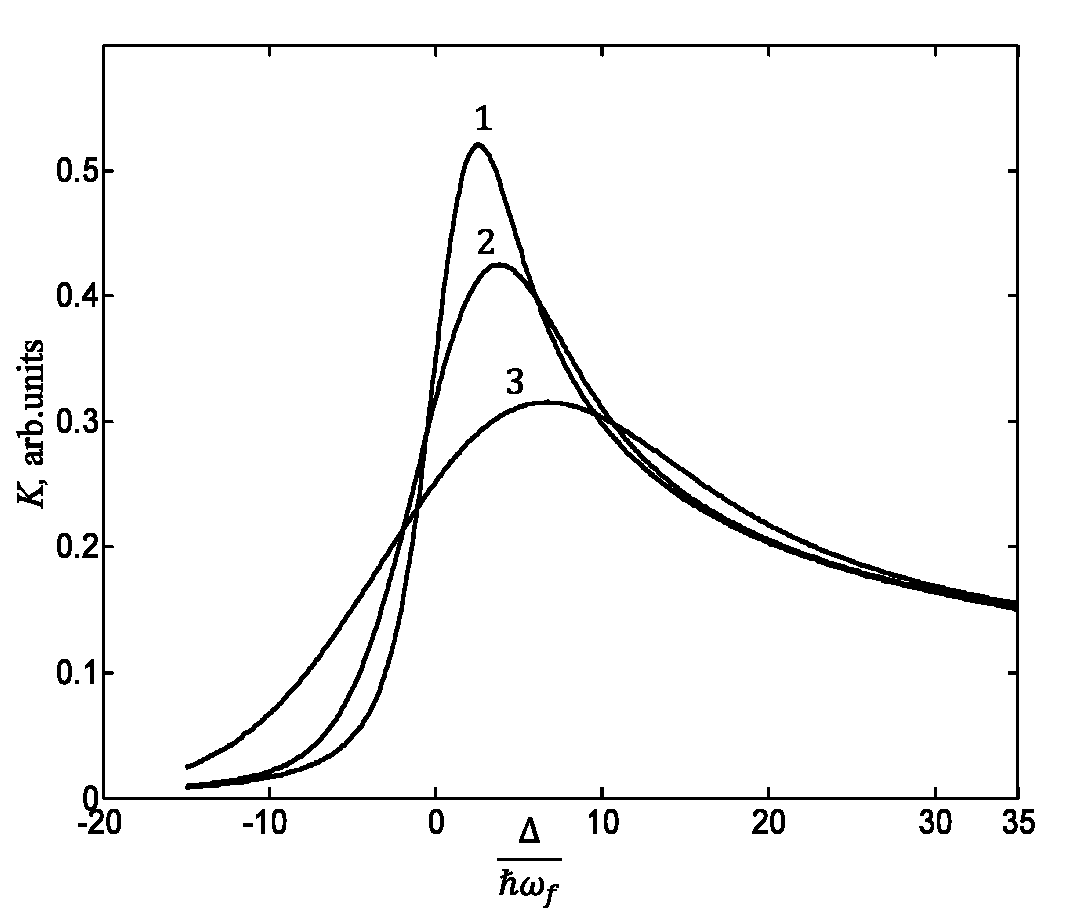
\includegraphics [scale=1] {fig_2_3_2}
	\caption{Зависимость первого пика межзонного поглощения света (в относительных единицах) от ${\Delta }/{\hbar {\omega }_f}$. Кривые 1, 2, 3 вычислены $\xi =0.25,\ \ 0.05,\ \ 0.01$ соответсвенно.} 
	\label{img:fig_2_3_2} 
\end{figure}

На рис. \ref{img:fig_2_3_2} представлена частотная зависимость коэффициента поглощения света (в относительных единицах) при различных значениях интенсивности лазерного излучения. Кривые 1, 2, 3 получены соответственно при$\xi =0.25,\ 0.05,\ 0.01$ $\left(\xi ={{\omega }^2_f}/{4a}\right).$ Как следует из рис. \ref{img:fig_2_3_2}, с ростом интенсивности ИК излучения ($\xi $ уменьшается при фиксированном значении ${\omega }_f$) форма линии поглощения изменяется: величина максимума поглощения уменьшается, а полуширина увеличивается. Заметим, что уже при $\xi \le 1$ коэффициент межзонного поглощения света полностью определяется интенсивностью ИК лазерного излучения.

Рассмотрим межзонное поглощение света в области второго пика магнетопоглощения (оптический переход II на рис. \ref{img:fig_2_3_1}) при ${\omega }_L=\Omega_e$ (магнито-инфракрасный резонанс). В этом случае коэффициент поглощения света согласно (3) при $m=0$, $n=1$ ($L_1\left(2at^2\right)=1-2at^2$) принимает следующий вид:

\begin{multline} \label{eq:23_70}
K\left(\Omega\right)=K_0{\left|\left\langle {\widetilde{\alpha }}_c\mathrel{\left|\vphantom{{\widetilde{\alpha }}_c {\widetilde{\alpha }}_v}\right.\kern-\nulldelimiterspace}{\widetilde{\alpha }}_v\right\rangle \right|}^2 4{\left[\frac{2{\mu }^*{\omega }_f}{\hbar a}\right]}^{\frac{1}{2}}\times\\
\times Re\int^{\infty }_0{dx}f\left(x\right)\left\{-\sqrt{\pi }f\left(x\right)e^{f^2\left(x\right)}\left[1-\Phi \left(f\left(x\right)\right)\right]+1\right\}
\end{multline} 
 
При $\xi ={{\omega }^2_f}/{4a}\gg 1$ (лазерное излучение отсутствует) из \eqref{eq:23_70} следует выражение для коэффициента поглощения слабой электромагнитной волны, полученное в \cite{Kostyukevich2015}. При $\xi <1$ (форма линии поглощения определяется интенсивностью резонансного ИК излучения) получено:
\begin{multline} \label{eq:23_80}
K\left(\Omega\right)=K_0{\left|\left\langle {\widetilde{\alpha }}_c\mathrel{\left|\vphantom{{\widetilde{\alpha }}_c {\widetilde{\alpha }}_v}\right.\kern-\nulldelimiterspace}{\widetilde{\alpha }}_v\right\rangle \right|}^2\pi z{\left[\frac{2{мì}^*\pi }{\hbar }{\left(\frac{8z}{a}\right)}^{1/2}\right]}^{1/2}e^{-z}\times\\
\times \left\{-\left[I_{3/4}\left(z\right)+\mathrm{sign}(\Delta) I_{-3/4}\left(z\right)\right]+\left(1+\frac{1}{4z}\right)\left[(I_{-1/4}\left(z\right)+ \mathrm{sign}(\Delta)  I_{1/4}\left(z\right)\right]\right\}
\end{multline}
\[
\mathrm{sign}(\Delta) = \begin{cases}
1,&\Delta >0 \\ 
-1,&\Delta <0
\end{cases}
\] 
%\[
%\mathrm{sign}\ \Delta =\left\{ \begin{array}{c}
%1,\Delta >0 \\ 
%-1,\Delta <0 \end{array}
%\right.
%\] 
$\left\langle {\widetilde{\alpha }}_c\mathrel{\left|\vphantom{{\widetilde{\alpha }}_c {\widetilde{\alpha }}_v}\right.\kern-\nulldelimiterspace}{\widetilde{\alpha }}_v\right\rangle $ -- матричный элемент сглаженных волновых функций носителей в возбужденном состоянии валентной зоны ($m=0$, $n=1$) и в возбужденном состоянии размерно-квантованной зоны проводимости.

\begin{figure}[ht] 
	\center
	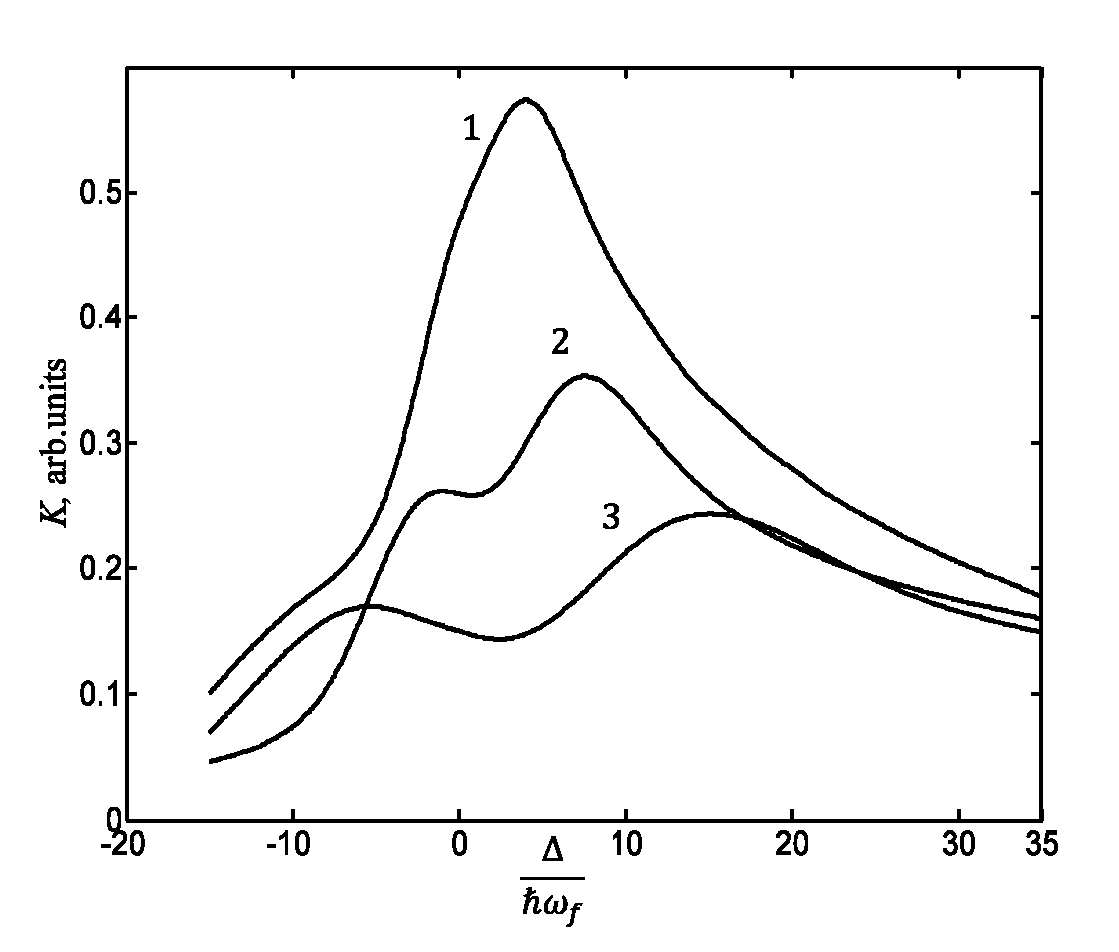
\includegraphics [scale=1] {fig_2_3_3}
	\caption{Зависимость второго пика магнетопоглощения (в относительных единицах) от ${\Delta }/{\hbar {\omega }_f}$ при различных значениях интенсивности резонансного $\left({\omega }_L=\Omega_e\right)$ лазерного излучения. Кривые 1, 2, 3 вычислены $\xi =0.25,\ \ 0.05,\ \ 0.01$ соответсвенно.} 
	\label{img:fig_2_3_3} 
\end{figure}

На рис. \ref{img:fig_2_3_3} приведена частотная зависимость второго пика магнетопоглощения при различных значениях $\xi $. Кривые 1, 2, 3 вычислены при $\xi =0.25,\ \ 0.05,\ \ 0.01$ соответсвенно. Как следует из рис. \ref{img:fig_2_3_3} с ростом напряженности E электрического поля пик магнетопоглощения (1) деформируется и при $\xi \ll 1$ расщепляется на два пика. При этом расстояние между ними и их полуширина увеличивается. Расщепление второго пика поглощения связано с тем, что при ${\omega }_L=\Omega_e$ возбужденное гибридное состояние ($n=1$) двукратно вырождено, и при взаимодействии с ИК лазерным излучением оно расщепляется. Эта ситуация близка к двойному оптическому резонансу (ДОР) на межзонных переходах в объемных материалах \cite{Perlin1970}.

Заметим, что $n$-пик магнетопоглощения расщепляется на n пиков. Если рассматривать случай z-поляризованной электромагнитной волны лазерного излучения, когда ${\omega }_L={\omega }_e$ (размерно-инфракрасный резонанс), то частотная зависимость коэффициента межзонного поглощения света (оптический переход III на рис. \ref{img:fig_2_3_1}) качественно не отличается от частотной зависимости, приведенной на рис. \ref{img:fig_2_3_2} и на рис. \ref{img:fig_2_3_3}.

Пусть при некотором значении напряженности электрического поля $E_c$ интенсивной электромагнитной волны вклад лазерного излучения в полуширину магнетоосцилляций примерно такой же как вклад, определяемый рассеянием носителей на шероховатой поверхности $\left(\xi =1\right)$. Естественно при $E_c<E$ форма линии межзонного поглощения слабой электромагнитной волны полностью определяется внешней лазерной подсветкой. Для типичных параметров полупроводниковой нанопроволоки $m_e=0.06m_0$, $m_v=0.4m_0$, $\sqrt[3]{{\gamma }_0}=20 \AA $ (такое значение $\sqrt[3]{{\gamma }_0}$ хорошо описывает большие значения подвижности $\mu \propto {10}^{4\ }\frac{cm^2}{V\cdot s}$, характерные для квантовых проволок) при $R_0={10}^3\ \AA $, $E_c=7\ \frac{V}{cm}$ для лазера H${}_{2}$O $\left(\hbar {\omega }_L=0.044\ eV\right)$. Следовательно, резонансное лазерное излучение заметно влияет на частотную зависимость межзонного поглощения света при небольших, вполне экспериментально доступных значений интенсивности ИК- лазерного излучения.
